% Generated by scripts/report-data.mjs. Do not edit.
\par\noindent\begin{minipage}{\linewidth}
\begin{center}
\definecolor{pc-P1}{HTML}{F17E7E}
\definecolor{pc-P2}{HTML}{7EF1A1}
\definecolor{pc-P3}{HTML}{C17EF1}
\definecolor{pc-P4}{HTML}{F1E37E}
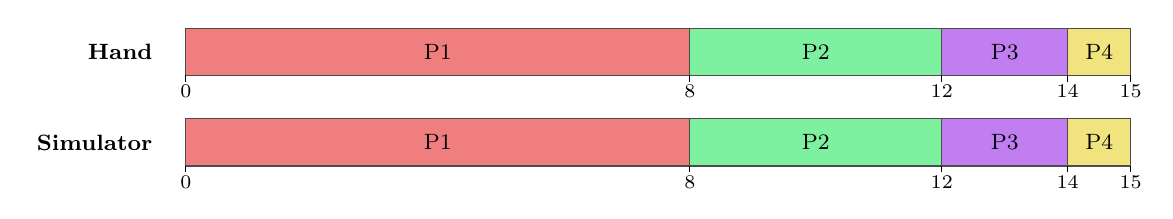
\begin{tikzpicture}[x=0.800cm, y=1cm, font=\footnotesize]
\node[anchor=east, font=\footnotesize\bfseries] at (-0.3/0.800, 0.3) {Hand};
\draw[fill=pc-P1, draw=black!70] (0, 0) rectangle (8, 0.6);
\node[align=center, inner sep=0pt] at (4, 0.3) {P1};
\draw[fill=pc-P2, draw=black!70] (8, 0) rectangle (12, 0.6);
\node[align=center, inner sep=0pt] at (10, 0.3) {P2};
\draw[fill=pc-P3, draw=black!70] (12, 0) rectangle (14, 0.6);
\node[align=center, inner sep=0pt] at (13, 0.3) {P3};
\draw[fill=pc-P4, draw=black!70] (14, 0) rectangle (15, 0.6);
\node[align=center, inner sep=0pt] at (14.5, 0.3) {P4};
\draw (0, 0) -- (0, -0.08) node[below, inner sep=1pt, font=\scriptsize] {0};
\draw (8, 0) -- (8, -0.08) node[below, inner sep=1pt, font=\scriptsize] {8};
\draw (12, 0) -- (12, -0.08) node[below, inner sep=1pt, font=\scriptsize] {12};
\draw (14, 0) -- (14, -0.08) node[below, inner sep=1pt, font=\scriptsize] {14};
\draw (15, 0) -- (15, -0.08) node[below, inner sep=1pt, font=\scriptsize] {15};
\node[anchor=east, font=\footnotesize\bfseries] at (-0.3/0.800, -0.85) {Simulator};
\draw[fill=pc-P1, draw=black!70] (0, -1.15) rectangle (8, -0.55);
\node[align=center, inner sep=0pt] at (4, -0.85) {P1};
\draw[fill=pc-P2, draw=black!70] (8, -1.15) rectangle (12, -0.55);
\node[align=center, inner sep=0pt] at (10, -0.85) {P2};
\draw[fill=pc-P3, draw=black!70] (12, -1.15) rectangle (14, -0.55);
\node[align=center, inner sep=0pt] at (13, -0.85) {P3};
\draw[fill=pc-P4, draw=black!70] (14, -1.15) rectangle (15, -0.55);
\node[align=center, inner sep=0pt] at (14.5, -0.85) {P4};
\draw (0, -1.15) -- (0, -1.23) node[below, inner sep=1pt, font=\scriptsize] {0};
\draw (8, -1.15) -- (8, -1.23) node[below, inner sep=1pt, font=\scriptsize] {8};
\draw (12, -1.15) -- (12, -1.23) node[below, inner sep=1pt, font=\scriptsize] {12};
\draw (14, -1.15) -- (14, -1.23) node[below, inner sep=1pt, font=\scriptsize] {14};
\draw (15, -1.15) -- (15, -1.23) node[below, inner sep=1pt, font=\scriptsize] {15};
\end{tikzpicture}
\end{center}
\begin{center}\small\setlength{\tabcolsep}{4pt}
\begin{tabular}{lcccccccccccc}
\toprule
 & & & \multicolumn{2}{c}{Start} & \multicolumn{2}{c}{Compl.} & \multicolumn{2}{c}{TAT} & \multicolumn{2}{c}{WT} & \multicolumn{2}{c}{RT} \\
\cmidrule(lr){4-5} \cmidrule(lr){6-7} \cmidrule(lr){8-9} \cmidrule(lr){10-11} \cmidrule(lr){12-13}
Proc. & Arr. & Burst & H & S & H & S & H & S & H & S & H & S \\
\midrule
P1 & 0 & 8 & 0 & 0 & 8 & 8 & 8 & 8 & 0 & 0 & 0 & 0 \\
P2 & 1 & 4 & 8 & 8 & 12 & 12 & 11 & 11 & 7 & 7 & 7 & 7 \\
P3 & 2 & 2 & 12 & 12 & 14 & 14 & 12 & 12 & 10 & 10 & 10 & 10 \\
P4 & 4 & 1 & 14 & 14 & 15 & 15 & 11 & 11 & 10 & 10 & 10 & 10 \\
\midrule
\multicolumn{7}{l}{Average (exact fractions)} & \multicolumn{2}{c}{42/4} & \multicolumn{2}{c}{27/4} & \multicolumn{2}{c}{27/4} \\
\bottomrule
\end{tabular}
\end{center}
\noindent\textbf{Comparison.} Hand (H) and simulator (S) agree on all 4 Gantt segments, all 20 per-process values and the 3 averages (turnaround 10.50 (42/4), waiting 6.75 (27/4), response 6.75 (27/4)). No discrepancy. The simulator's 5 invariants: 5/5 pass.
\end{minipage}\par\medskip
